\documentclass[11  pt]{article} 
\usepackage[lmargin=1in,rmargin=1.75in,bmargin=1in,tmargin=1in]{geometry}  


\input{preamble}

\begin{document}
	\week{10b: Computational Complexity}{March 26, 2026}
	
	\paragraph{Course Logistics}
	\begin{itemize}
		\item Exam 2 next Thursday
		\item Review session next Tuesday
		\end{itemize}
	
	
	\section{Views of the computational problem universe}
	There are four different possibilities for the relationship between P, NP, and co-NP.
	
	
	
	\vfill
	
	There are two possibilities for the relationship between P, NP, and NP-complete.
	
	\vfill
	
	\newpage
	
	\paragraph{A few famous NP-complete problems}
	\begin{itemize}
		\item Find if a graph has a clique of size at least $k$
		\item Find if a graph has a Hamiltonian cycle
		\item Find if a graph has a simple path with at least $k$ edges
		\item \textbf{Subset sum}: given a set of numbers, find if any subset sums to zero
		\item \textbf{SAT}: Logic problems we will look at in more depth later
	\end{itemize}
	
	
	\section{Summary on Reduction and NP-completeness}
	If $A$ can be reduced in polynomial time to $B$, we write $A \leq_p B$. This means that $A$ is no harder than B; a solver for $B$ can be used to solve $A$.\\
	
	\vs{2cm}
	\vfill
	
	A problem $Q$ is NP-hard if every problem in NP can be reduced to $Q$ in polynomial time. \\
	
	A problem $Q$ is NP-complete if
	\begin{itemize}
		\item It is in NP
		\item It is NP-hard\\
	\end{itemize}
	
	\vfill
	
	
	\begin{Qu}
		Assume that $A$ and $B$ are both in NP and $A \leq_p B$. Which of the following statements is false?
		\begin{itemize}
			\aitem If $A \in \text{P}$, then $B \in \text{P}$
			\bitem If $A$ is NP-complete, then $B$ is NP-complete
			\citem If $B \in \text{P}$, then $A \in \text{P}$
			\ditem If $A$ is NP-complete, then $B \leq_p A$
		\end{itemize}
	\end{Qu}
	\vs{1cm}
	
	If two problems are NP-complete, then they are both in NP, and:
	
	\vs{1cm}
	
	\newpage
	
	\section{Why does it matter whether a problem is in P, NP, or is NP-complete?}
	%There are lots of problems we want to know how to solve with a computer. When we encounter a new problem, it's helpful to know how inherently challenging the problem is! \\
	
	A famous book by Garey and Johnson, \emph{Computers and Intractability}, includes some famous cartoons to help us answer this question.\footnote{Garey, Michael R., and David S. Johnson. Computers and intractability. Vol. 174. San Francisco: freeman, 1979. High-resolution versions of the cartoon are available online. }\\
	
	Let's say your boss tells you that because you are a CS major or minor you should be able to find an efficient algorithm for a certain problem at work. You work for weeks without progress. You don't want to tell your boss:
	
	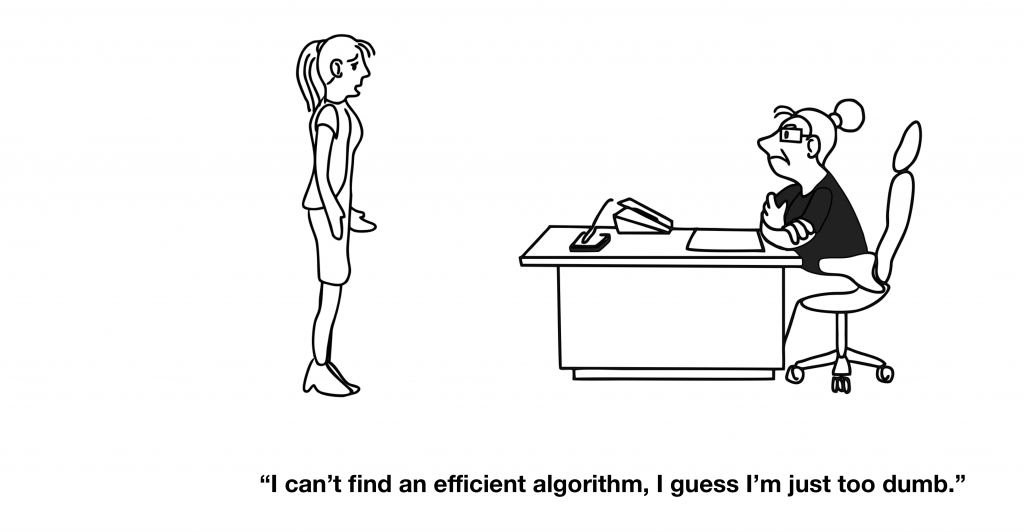
\includegraphics[width=\linewidth]{cartoon.png}
	
	Ideally you'd like to be able to say:
	
	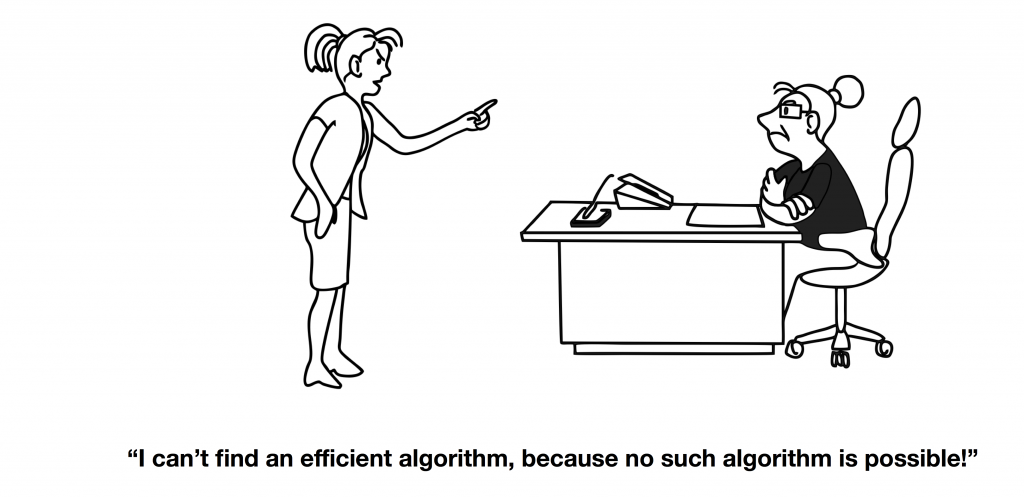
\includegraphics[width=\linewidth]{cartoon2.png}
	
	But in most situations, proving definitively that this is impossible is unlikely.
	\newpage
	
	If you fail to find an efficient solution to a problem, ask yourself: am I struggling to find a solution simply because this is NP-complete? If you can prove it is, you have a great answer for your boss.\\
	
	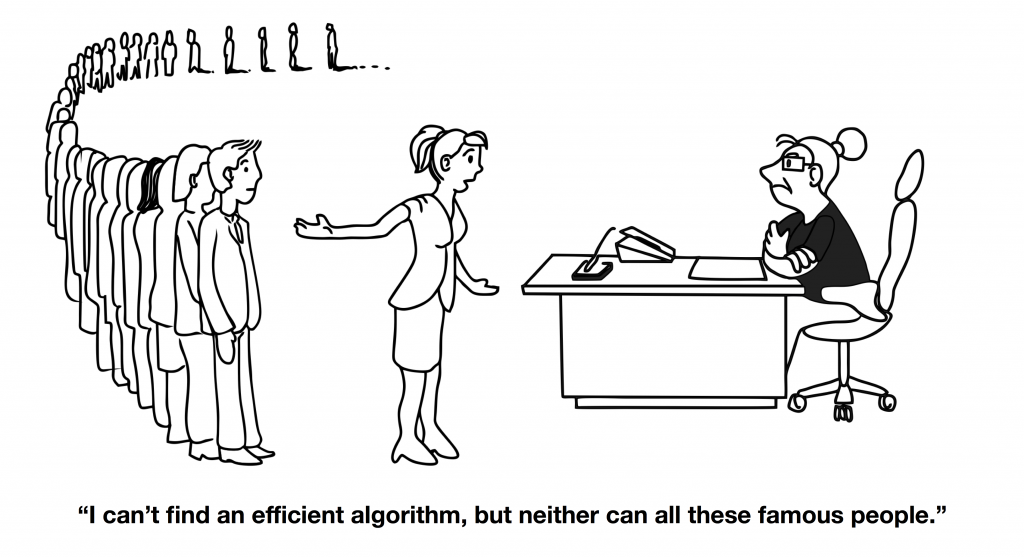
\includegraphics[width=\linewidth]{cartoon3.png}
	
	
	\section{A brief and incomplete history of NP-completeness}
	
	\begin{itemize}
		\item 1971: Stephen Cook proves that every problem in NP can be reduced to a problem called \emph{Boolean Satisfiability} (SAT).\\
		
		In modern terminology: SAT is NP-complete.\\
		
		The same results were developed independently by someone named Leonid Levin, so this is now called the \emph{Cook-Levin} Theorem. \\
		\item 1972: Richard Karp publishes a paper \emph{Reducibility Among Combinatorial Problems}, showing that SAT can be reduced to 21 other problems. \\
		
		
		\item 1979: Garey and Johnson publish the go-to reference on NP-completeness: \emph{Computers and Intractability}.
	\end{itemize}
	
	\section{Boolean Satisfiability Problems}
	A \emph{boolean variable} is a variable $x$ that can take on the values True or False. \\
	
	A \emph{boolean expression} or \emph{boolean formula} is built from 
	\begin{itemize}
		\item Variables: $x_1, x_2, \hdots , x_n$, all in $\{\text{True}, \text{False}\}$ \\
		\item Operators: 
		\begin{itemize}
			\item AND ($\land$): e.g., True $\land$ False = False\\
			\vs{1cm}
			
%			\emph{Returns true if and only if both operands are true.}\\
			
			\item OR ($\lor$):  e.g., True $\lor$ False = True \\
						\vs{1cm}
%			\emph{Returns true only if either operand is true; false otherwise.}
			\item NOT: $\neg \text{True} = \text{False}$; $\neg \text{False} = \text{True}$ \\
			
			This is often also denoted with an overline: \\ \\%$\neg \text{True} = \overline{\text{True}}$; $\bar{0} = 1$.
		\end{itemize}
		\item Parentheses: telling you the order in which to evaluate statements
	\end{itemize}
	\vfill
	
	Here are some examples of Boolean expressions:
	\begin{itemize}
		\item $x_1 \land x_2 \land x_3$
		\item $\neg x_2 \lor x_3$
		\item $(\neg x_1 \land x_2) \lor (x_1 \land x_2 \land x_3) \lor (x_2 \lor x_3)$
	\end{itemize}
	\vfill
	\newpage
	
	\begin{Qu}
		Does the following statement evaluate to True or False?
		$$(T \land F) \lor (T \land F \land T) \lor (F \lor T)$$
		\begin{itemize}
			\aitem True
			\bitem False
		\end{itemize}
	\end{Qu}
	\vfill
	\begin{Qu}
		Is the following Boolean expression satisfiable or not?
		$$(x_1 \land x_2) \lor (x_1 \land x_2 \land x_3) \lor (\neg x_1 \lor x_3)$$
		\begin{itemize}
			\aitem Yes, it's satisfiable
			\bitem No, it's not satisfiable
		\end{itemize}
	\end{Qu}
\vfill
	\newpage
	
	
	\begin{theorem} Checking whether a boolean formula is satisfiable is \hide{NP-complete.}
	\end{theorem}
	We will not prove this, but we'll use it as a starting point for proving other problems are NP-complete.
	
	\section{CNF Satisfiability and 3SAT}
	
	Some more terminology
	\begin{itemize}
		\item Literal: a boolean variable or its negation: e.g., \\ \\ 
		\item Clause: the OR of multiple literals: e.g., \\ \\
		\item A boolean formula is in conjunctive normal form if it is the AND of clauses. \\
		
		
	\end{itemize}
	\vs{3cm}
	
	
	A boolean formula is in 3-CNF if \hide{all clauses have exactly 3 literals.}
	
	\vs{5cm}
	
	
	
	\begin{theorem} Checking whether a boolean formula in 3-CNF is satisfiable is NP-complete. This is called 3SAT.
	\end{theorem}
	Again: we'll use it as a starting point for proving other problems are NP-complete.
	
%\newpage
%	\section{Reduction Example}
%
%\begin{theorem}
%	$\textsc{Clique}(G,k)$ can be reduced to SAT.
%\end{theorem}
%\textbf{Proof.} Start with $G = (V,E)$, with node set $V = \{v_1,v_2, v_3, \hdots , v_n\}$. To find a clique of size $k$, we need to assign nodes in $V$ to $k$ different ``clique node'' positions
%\vspace{2cm}
%
%
%Define a variable $x_{v,i}$ as follows:
%
%\vspace{3cm}
%
%To convert a \textsc{Clique} instance into an instance of SAT, we must realize that finding a clique is equivalent to satisfying the following properties when assigning nodes in $V$ to be ``clique nodes.''
%
%\begin{itemize}
%	\item Each ``clique node'' position must be filled.
%	\vspace{3cm}
%	\item A node $v \in V$ can be assigned to at most one clique node position.
%	\vspace{3cm}
%	\item Every pair of nodes $\{u,v\}$ assigned to be clique nodes must share an edge.
%\end{itemize}


	\newpage
	
\section{The clique problem is NP-complete}
\textbf{The clique problem:} Check if an unweighted and undirected graph $G = (V,E)$ has a clique of size $k$. Formally we write this as:

\begin{center}
	\textsc{Clique} = $\{\langle G,k \rangle \colon \text{$G$ has a clique size $k$} \}$\\
\end{center}

\begin{theorem}
	The clique problem is \hide{NP-complete.}
\end{theorem}
Proof structure:
\begin{itemize}
	\item We have already shown the problem \hide{is in NP.}
	\item We will show how to reduce every 3SAT problem to a clique problem.
	\item We will show that a YES instance of 3SAT is a YES instance of clique
	\item We will show that a YES instance of clique maps to a YES instance of 3SAT
\end{itemize}
\newpage

%\paragraph{Proof}
\textbf{The reduction.} Consider an arbitrary instance of 3SAT, and let $k$ be the number of 3-clauses it contains, denoted by
\begin{equation}
	C_1 \land C_2 \land \cdots \land C_k
\end{equation}
For $r  \in \{1,2, \hdots k\}$, let the literals in the $r$th clause be denoted as $l_1^r, l_2^r, l_3^r$ so that: 
\begin{equation}
	C_r = (l_1^r \lor l_2^r \lor l_3^r)
\end{equation}
In other words, $l_i^r$ is the $i$th literal in the $r$th clause.\\

For each literal $l_i^r$, we introduce a node $v_i^r$. \\


For each pair of literals $\{l_i^r, l_j^s\}$, we add an edge $(v_i^r, v_j^s)$ if:
\begin{itemize}
	\item $r \neq s$ 
	\item $v_i^r$ is not the negation of $v_j^s$; this means they are \emph{consistent}
\end{itemize}

\paragraph{Let's consider an example} $(x_1 \lor \overline{x}_2 \lor \overline{x}_3) \land (\overline{x}_1 \lor x_2 \lor x_3) \land (x_1 \lor x_2 \lor x_3)$

\newpage
\textbf{The rest of the proof:} We need to prove that YES for the 3SAT instance maps to YES for the clique instance, and that NO for the 3SAT instance maps to NO for the clique instance.\\

This is equivalent to proving that the 3SAT instance is satisfiable if 

\vs{2cm}


It turns out this is true but we will not prove it. The outline of the proof is:

\begin{itemize}
	\item $(\implies)$ Assume there is a satisfying assignment, and prove that the literals set to TRUE to satisfy the $k$ clauses map to \\ \\
	\item $(\Longleftarrow)$ Assume that there is a $k$-clique in the reduced graph and prove that 
\end{itemize}


\newpage

\section{The 2SAT Problem}
Similar to 3SAT, the problem 2SAT is the task of finding a satisfying assignment for a boolean satisfiability formula in conjunctive normal form (an AND of ORs) when all clauses involve exactly two literals. \\


\vspace{3cm}


\begin{Qu}
	Consider the following two true facts. \\
	
	\textbf{Fact 1:} Every instance of 2SAT is an instance of SAT. \\
	
	\textbf{Fact 2:} You can reduce 2SAT to \textsc{Clique}, similar to the way we reduced 3SAT to \textsc{Clique}\\
	
	Which of the following statements is true?
	\begin{itemize}
		\aitem Fact 1 implies that 2SAT is NP-hard, but Fact 2 does not
		\bitem Fact 2 implies that 2SAT is NP-hard, but Fact 1 does not
		\citem Both facts imply that 2SAT is NP-hard
		\ditem Neither fact is sufficient to conclude that 2SAT is NP-hard
	\end{itemize}	
\end{Qu}


\newpage
\section{Another reduction for 2SAT}

Given an instance of 2SAT, construct the \emph{implication graph} as follows:
\begin{itemize}
	\item Create a node for each variable and its negation
	\item For a clause $(\ell_1 \lor \ell_2)$ (which may be positive or negative literals), add:
	\begin{itemize}
		\item A directed edge $(\neg \ell_1, \ell_2)$
		\item A directed edge $(\neg \ell_2, \ell_1$)
	\end{itemize}
\end{itemize}

\textbf{An example.}

\begin{center}
 {\Large $(x_1 \lor x_2) \land (x_1 \lor \overline{x}_3) \land (\overline{x}_2 \lor x_3) \land (x_4 \lor \overline{x}_3) \land (\overline{x}_1 \lor \overline{x}_3)$}
 \end{center}
\vs{4cm}

\newpage
\begin{theorem}
	In the implication graph for the 2SAT instance, a variable and its negation will be in separate strongly connected components if and only if % the 2SAT problem has a satisfying solution.
\end{theorem}



\end{document}